\subsection{Datasets used} \label{s:lit:datasets_used}

There are two important types of datasets used in the project: the gene expression of non-cancerous bladder from The Jack Birch Unit for Molecular Carcinogenesis (The University of York, UK) and the MIBC cohort from \acrlong{tcga}. The JBU data is currently in the process of getting published\footnote{In the near future after this PhD is completed, the data is likely to become available on a public portal} as the dataset helps building a representation of the urothelium it closely resembles the healthy tissue, throughout the project the JBU dataset is refereed as non-tumour, healthy or non-cancerous dataset. The TCGA dataset is publicly available from the Genomics Data Central (GDC) portal\footnote{A new user needs to set an agreement with the Genome Data Comons in order to have access \url{https://portal.gdc.cancer.gov/}}.

Both gene expression datasets used in this project were pseudo-align using the Kallisto method\citep{Bray2016-cv} and genome version GRCh38 with Gencode annotation version 42 which resulted in $\sim33k$ genes for each dataset.

\subsubsection*{The healthy dataset} \label{s:lit:non_tum_data}

Taking a bladder biopsy is an invasive procedure making it challenging to obtain samples from completely healthy patients, thus benign diseases were used to form a non-tuorm molecular representation of the bladder. These samples included \acrfull{oab}, \acrfull{sui}, \acrfull{nvh}, post-prolapse staging, survey after a \acrfull{tvt} procedure, and other abnormal conditions such as \acrfull{cc} and a patient suffering with \acrfull{ruti}. Consequently, the dataset includes samples where the urothelium should be completely normal (backed up by histology) such as \acrshort{oab} and \acrshort{sui}, but also those with active pathology such as \acrshort{cc} or \acrshort{ruti}.

The non-cancerous dataset from JBU comprised 88 samples, of which 49 are ABS-Ca differentiated, 23 are freshly isolated (P0), and 14 are Undifferentiated (UD). \Cref{fig:lit:diff_samples} illustrates the different stages of tissue sample processing, where the cells separated from stroma represent the bladder's closest representation, \gls{P0} samples. Isolated cells grown as a monoculture on plastic de-differentiate and become highly proliferative with growth regulated by \textit{EGFR}, a pathway shut off in differentiated cells and reactivated in growth-unrestricted bladder cancers. These cells can be re-differentiated from a biomimetic urothelium by changing the growth medium to contain 5\% Adult bovine serum (ABS) and increasing the Ca2+ concentration to physiological levels \citep{Cross2005-fe}. Histologically, these re-differentiated tissues are highly analogous to freshly isolated (P0) tissues but enable the study of urothelial molecular machinery in the absence of extrinsic factors, which may still impact P0 samples. Together, these represent three distinct, informative and cancer-relevant urothelial states, but it should be noted that they do not represent the limit of urothelial transcriptomic plasticity.

% After the biopsies are collected, the urothelium is separated from the stroma and the cells are segregated, resulting in freshly isolated cells or \acrshort{p0}. To obtain \acrfull{ud} cells, the protocol from \citet{Cross2005-fe} is used. To create a biomimetic tissue, the \acrshort{abs} differentiation protocol described by \citet{Cross2005-fe} is employed in the fourth step.

% Aspects of the three differentiation status
The \gls{ABSCA} samples were grown in the lab to exhibit the 'purer' markers of the urothelium differentiation and molecular properties of the healthy bladder tissue. The P0 samples exhibit the differentiation markers as in the ABS-Ca differentiated tissues as well as some cell infiltration aspects, offering a more realistic molecular representation of the bladder tissue. 

% Linking to TCGA
By their differentiation status both ABS-Ca and P0 are closer to Luminal samples in the MIBC. As undifferentiated urothelial cells, \gls{UD} transcriptomes are closer to basal MIBC subtypes. These aspects are observed in the analysis performed in the selective edge pruning (\cref{s:N_I:sel_pruning}) and in the work with the refined version of the network pipeline in (\cref{s:N_II:std_net}).

\begin{figure}[!b]
    \centering
    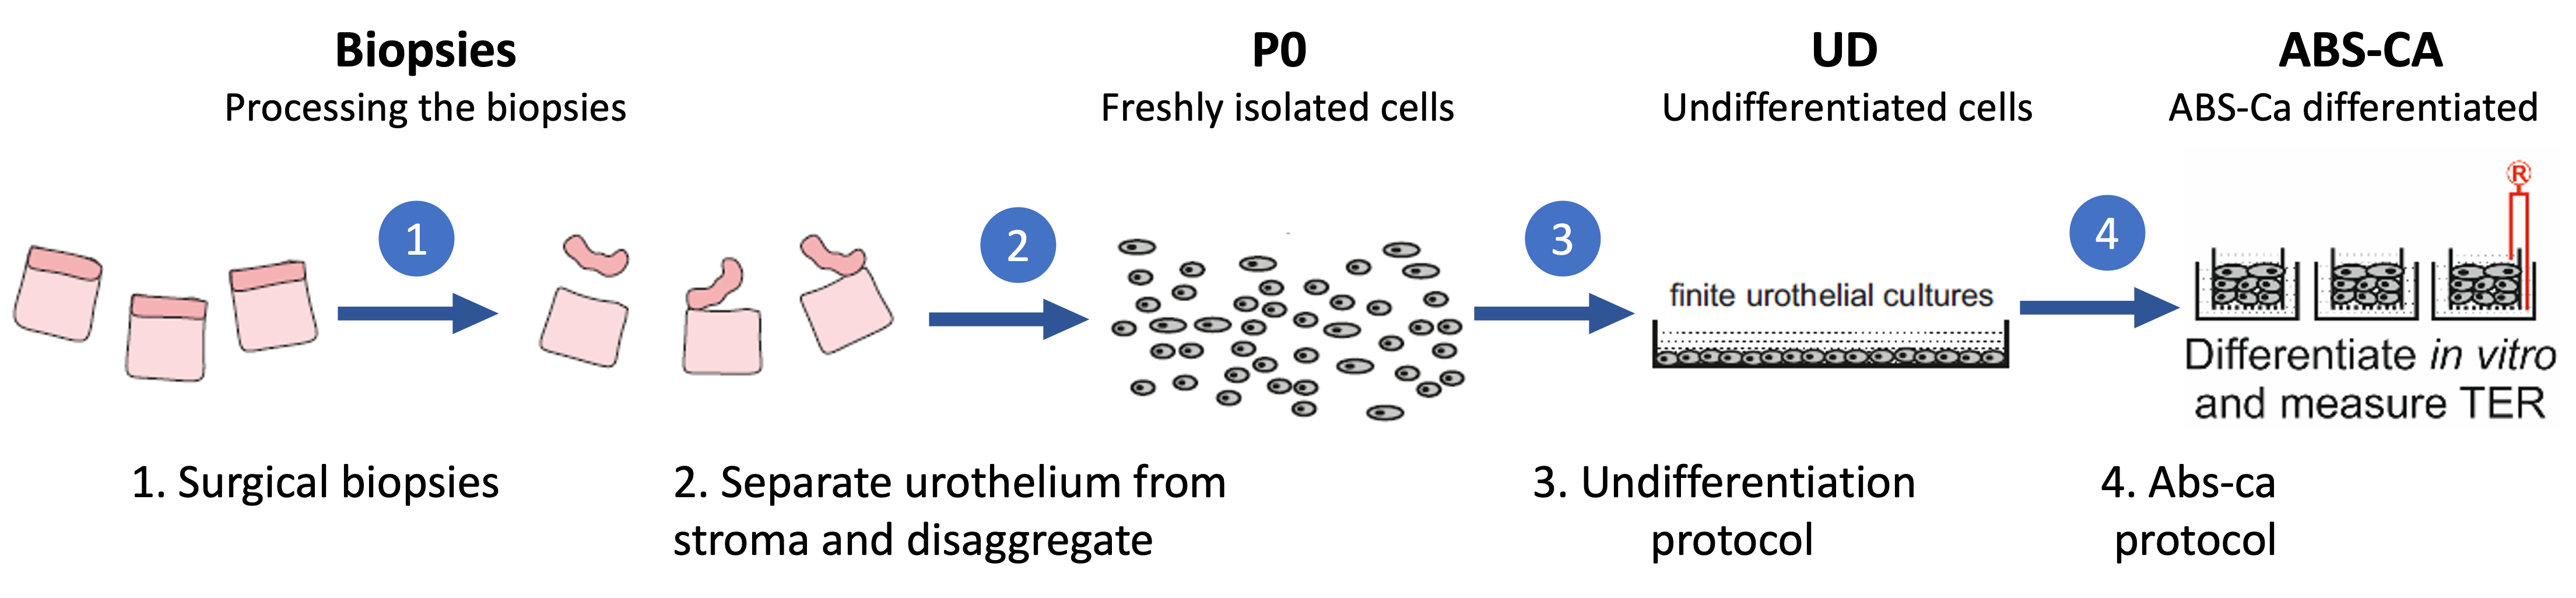
\includegraphics[width=1.0\textwidth, keepaspectratio]{Sections/Lit_review/Resources/differentiation.png}
    \caption[Bladder samples protcol for the healthy dataset]{Overview of the processing of bladder tissue samples forming the non-tumour dataset from \acrfull{jbu}. After the collection of biopsies, the samples are processed to separate the urothelium from the stroma, resulting in freshly isolated cells (P0). To obtain undifferentiated cells (UD), the protocol described by \citet{Cross2005-fe} is used. These cells can then be used to create biomimetic tissue using the ABS-Ca protocol described in \citet{Cross2005-fe}.}
    \label{fig:lit:diff_samples}
\end{figure}


% Where this is used
In this project three different networks are created using the P0 and analysed in \cref{s:p0}, with the goal to inform the stratification of the \acrshort{mibc} using the molecular representation of freshly isolated cells. However, the P0 samples do not represent the Basal tumour samples which are closer to the  undifferentiated tissue state, and the research in \cref{s:N_II} utilised both the gene expressions from UD samples and the additional differentiated tissue samples with ABS-Ca.

\subsubsection*{The Cancer Genome Atlas} \label{s:lit:tcga_data}

The \acrshort{mibc} cohort from \acrfull{tcga} is central in this project, contributing with the gene expressions from \gls{RNASEQ} and the somatic mutations from \gls{WES} (WES) to all the results chapters.  The WES data was filtered and only non-synonymous mutations (Frameshift, Nonsense and Missense) are included as these have the potential to cause changes in the protein. The metadata available is used to compute the different survival rates for the subtypes derived across the project, see method in \cref{s:lit:survival}, and the cell infiltration analysis in \cref{fig:cs:tumour_purity}.
